\RequirePackage{luatex85,shellesc}
\documentclass[a4paper,9pt, addpoints, solutions]{exam}
\usepackage{pgf,tikz}
\usetikzlibrary{shapes.geometric}
\usepackage{tikzsymbols}
\usepackage{marginnote}
\usepackage{pgfplots}
\usepackage{caption}
\usepackage{booktabs}
\usepackage{grffile}
\usepackage{amsmath}
% \linespread{1.1}
\usepackage{mathtools}
\usepackage{amssymb}
\usepackage{tcolorbox}
\usepackage{fontspec}
\setmainfont{opensans}
\usepackage[euler-digits]{eulervm}
\usepackage{pgfplots}
\usepackage{epsdice}
\usepackage{tfrupee}
\usepackage[top=2cm, bottom=2cm, left=3cm, right=5cm, heightrounded,
      marginparwidth=4cm, marginparsep=5mm]{geometry}


\newcommand\MEAN[1]{\langle #1\rangle}
\newcommand\VAR[1]{\text{Var}(#1)}
\newcommand\BONUS{\textbf{(bonus)} }
\newcommand\MARGIN[1]{\marginpar{\emph{\small #1}}}

% Title Page
\title{Information Theory 2019 \\ Tutorial 1} 
\date{\today}
\begin{document}
\maketitle

\section{Probability}

\begin{itemize}
    \item $\Omega$ : Set of all possible outcome.
    \item $Pr(x)$, probability of event $x$. $x$ must be in $\Omega$ (i.e., $x \in \Omega$).
    \item  Sum of $Pr(x)$ for all $x$ in $\Omega$ must add to to 1 or,
        mathematically, $\sum_{x\in\Omega} Pr(x)= 1$ \footnote{You will see
        $\sum$ more often in the course. Familiarize yourself with $\sum$}
\end{itemize}

For example, when I roll a die it can land in six ways. For such a  die,
$\Omega$ consists of six outcomes (elements).  $\Omega={ \epsdice{1},
\epsdice{2}, \epsdice{3},\epsdice{4},\epsdice{5},\epsdice{6} }$. When die is
fair, all outcomes are equally likely i.e. $Pr(\epsdice{1}) = Pr(\epsdice{2}) =
\ldots = Pr(\epsdice{6})$. Also $Pr(\epsdice{1}) + Pr(\epsdice{2}) + \ldots +
Pr(\epsdice{6}) = 1$. These two facts implies that any outcome has the
probability of $\frac{1}{6}$ or $Pr(x) = \frac{1}{6}$,  $\forall x\in\Omega$
($\forall$ is shorthand for `for all').

\paragraph{Mean and Variance} There are three prominent ways to compute/estimate
the 'average': mean, mode and median. We'll focus on mean here since it turns
out to be the more meaningful in applications than the rest. Mean is also called
expected value \MARGIN{I get it: On average, ``average'' means ``mean''}.  For a random
variable $X$, we shall use the symbol $\MEAN{X}$ to denote the mean (expected
value) of it. The variance of $X$ (often denoted by $\VAR{X}$) is the measure of
variability in the random variable $X$. It is defined as the mean square
deviation from the mean. $\VAR{X} = \MEAN{X - \MEAN{X}}^2$ (see problem 2).

Two random variables $X$ and $Y$ are called independent if the output of one
does not depend on the outcome of other. 

\subsection*{Problems}
\begin{questions}

    \question Mean and variance
    \begin{parts}
        \part[1] What is the expected value of a pair of dice.
        \part[5] Why do we care about variance? Everyone computes it but what is
        so natural about it? (Hint: $Pr\left((X-\MEAN{X})^2 \ge \alpha \right) \le
        \VAR{X}/\alpha$ [Chebyshev 1963]) 
    \end{parts}

\question[5] Prove of disprove: If $X$ and $Y$ are independent random variables,
then so are $F(X)$ and $G(Y)$ where $F$ and $G$ are any function. [Concrete
Math, Graham et al.]

\question[3] \BONUS Construct a random variable which has finite mean and infinite
variance.

\question[10]
Two lotteries sells 100 tickets every week. At the end of the week, one of these
tickets is selected randomly (each ticket is equally likely to win) and winner
is given 1 lakh rupees. Other 99 tickes gets nothing. You have enough money to
buy two tickets: you can buy both tickets from the same lottery or 1 from each
lotteries. Which strategy is \textit{better} given that you can play lottery enough
time.

\begin{solution} 
    If we buy two tickets from the same lottery (strategy \textbf{S1}), we have
    2% chance of winning \rupee 1 lakh, and 98% change of winning nothing.  If
    we buy both tickets from different lotteries (strategy \textbf{S2}), we have
    some change of winning \rupee 2 lakhs. Lets write down the probabilities.

    \begin{tabular}{c c c c}
        Strategy                    & \rupee 0     & \rupee 1 lakh & \rupee 2 lakh \\
        S1                          & 0.98         & 0.02          & \\
        S2                          & 0.9801       & 0.0198        & 0.0001 \\
    \end{tabular}

    With S2, we have slightly higher chance of not winning anything. But a non-zero
    chance of winning \rupee 2 lakhs. The expected value of win (mean) is same is
    both cases: $0 \times 0.98 + 0.02 \times 1 = 0.02$, and $0\times 0.9801 + 0.0198
    * 1 + 0.0001 * 2 = 0.02$. Yet the strategy looks different. After all if I buy
    100 tickets from same lottery, I am sure to win \rupee 1 lakh, but not with S2.

    Strictly speaker, which strategy is better is beyound the scope of this
    tutorial. All we can show how to do the calculations.  The standard deviation of
    S1 is ($\sqrt{0.98(0-0.02)^2+0.02(1-0.02)^2}$) 0.1386 and of S2 is
    0.1392265. We can say that S2 is \rupee 0.0006265 lakh riskier.

    Let play this lottery on computer since we can not play in real life.
    Figure @fig:1 shows the simultion. More often than not, S2 gives slightly
    higher return.

        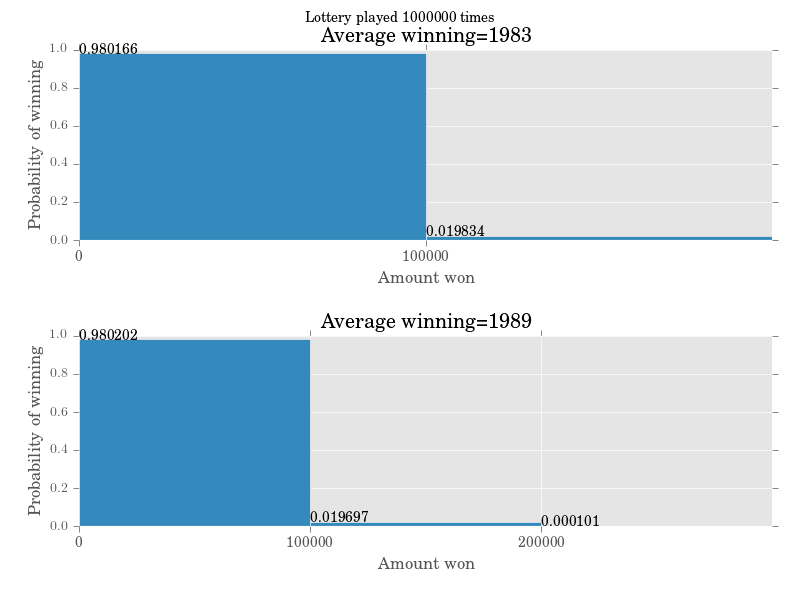
\includegraphics[width=1\textwidth]{./lotteries.py.png}
        \captionof{figure}{Second strategy is slightly better. On average, we might win more
            money with S2 given that we win \rupee 2 lakh. For very large number (almost
            infinite), both strategy will yield same results (since mean is same), however
            for large numbers of times lottery played, S2 seems to be more beneficial (as
        per simulations).}
        \label{fig:lottery}
\end{solution}

\question For a pair of dice, write $\Omega$.
\begin{parts}
    \part[2] Consider $\epsdice{1}\epsdice{4}$ and $\epsdice{4}\epsdice{1}$ etc. as distinct events.
    \part[3] Consider $\epsdice{1}\epsdice{5}$ and $\epsdice{5}\epsdice{1}$ etc. as same event.
    \part[3] \textbf{(bonus)} Repeat the problem for 4 dice. You can use computer program to
check your results.
\end{parts}

\question[5]
Your TA flipped a Rs. 1 coin repeatedly. Once he got two head in succession,
he noted down the number of flips. He got the following sequence:
\verb|6,3,6,8,7,12,16,2,3,2| 
Fortunately others have also done such excercise. I was able to get following
data from two universities.

\verb|3,2,3,5,10,2,6,6,9,2|     (Stanford, 1979)
\verb|10,2,10,7,5,2,10,6,10,2|  (Princeton, 1987)

\begin{parts}
    \part[2] Compute (umm. estimate) the mean and variance of these sequences.
    \part[3] \textbf{(bonus)} Based on these sequence, can you estimate the
    probability that coin used was not 'fair'? If yes, estimate. If no, why not?
\end{parts}

\begin{solution}
\begin{tabular}{c c  c}
 Coin         & mean & $\sqrt{\text{variance}}$ \\
NCBS 2017     & 6.5  & 4.34  \\
Stanford 1979 & 4.79 & 2.78  \\
Princeton 1987& 6.4  & 3.35  \\
\end{tabular}

The answer is no and its not easy to explain.
Lets call this process X. Lets take an extreme case: NCBS 2017 series was the
following: 2,2,2,2,2,2,2,2,2,2 i.e. all 20 flips gave us heads. Can we say this
was definately a loaded coin? What is the probability that this sequence came
out of a fair coin? Or what is the probability of getting 20 heads in
succession? Ans is $(\frac{1}{2})^{20}$. It is non-zero!

What is the mean and variance of X for a fair coin anyway?  \footnote{mean=6,std=4.7}
\end{solution} 

\question[10] \textbf{Ultimate Frisbee} 
Six (five) players stand at the vertices of a hexagon (pentagon), throwing
Frisbees to each other.

\tikz{
    \node[draw, regular polygon, blue, regular polygon sides=6, inner sep=1cm] (a) {};

    \tikzset{frisbee/.style={-latex, very thick, shorten <= 2pt}}
    \node[circle, fill=blue] (p1) at (a.corner 1) {};
    \node[circle, fill=blue] (p2) at (a.corner 2) {};

    \draw[frisbee] ([shift=(45:1mm)]p1) -- ++(-60:7mm);
    \draw[frisbee] ([shift=(45:1mm)]p1) -- ++(-180:7mm);

    \draw[frisbee] ([shift=(45:1mm)]p2) -- ++(0:7mm);
    \draw[frisbee] ([shift=(45:1mm)]p2) -- ++(-135:7mm);
}

They have two Frisbees, initially at the adjacent vertices as shown in the
figure above. The Frisbee is thrown either to the left or to the right with
equal probability. The game stops when one player is the target of both
Frisbees. (All throws the independent of past history).

\begin{enumerate}
    \item Find the mean and variance of the number of pairs of throws. For some
        initial values, the game may never stop in the case of hexagon.
    \item Find the expression for probability that the game lasts more than 500
        steps, in terms of Fibonacci numbers.
\end{enumerate} [Coc. Math., Knuth]

\paragraph{Typical dressing}

\question[5] \textbf{(Counting)}
A man has a non-magical wardrobe containing 10 shirts, 10 pants, 20 pairs of
socks, 10 pairs of shoes, 30 hats, and 50 neck-ties. He picks 6 items everyday.
Whenever he picks 1 shirt, 1 pant, 1 pair of shoes, 1 pair of socks, 1 hat and
1 neck-tie, we call is 'typical dressing'.

\begin{parts}
    \part[2] How many ways he can choose 6 items? 
    \begin{solution}
        There are total 130 items.  For first item, we have 130 choices,
        for second item, we have 129 choices etc. Total choices are $130 \times 129
        \times 128 \ldots 125$.
    \end{solution}

    \part[3]How many ways he can dress himself 'typically'?
    \begin{solution}
        He has to pick 1 items of each type. How many ways he can choose 1
        shirt out of 10 shirts? 10. Similarly there are 30 ways to pick 30 hats etc.
        Total typical dressings are $10 \times 10 \times 20 \times 10 \times 30 \times
        50$.
    \end{solution}

    \part[3] In a slightly off-beat world, a typical dressing contains at least 1
    shirt, 1 pant, and 1 pair of shoes. Rest of the 6 garments could be
    anything else. How many ways he can dress himself 'typically'?
    \begin{solution}
        Let assume that he picks required 1 shirt first. There are 10 ways. Next he
        picks required 1 pant, there are 10 ways. Similarly there are 10 ways for
        picking required 1 pair of shoes. Left are 3 garments and they could be anything.
        How many ways he can pick 3 items out of 9 shirts, 9 pants, 10 pairs of shoes,
        20 pairs of socks, 30 hats and 50 neck-ties (total 127). Go back to problem 1. Ans is 
        $127 \times 126 \times 125$ for this part. So total ways to dress oneself
        typically is $10 \times 10 \times 10 \times 127 \times 126 \times 125$.
    \end{solution}
\end{parts}

\section{Distributions} \question[5] A man claims that he has average height and
average weight, therefore, he is an average man. But he is considered slightly
overweight. Explain? (Hint: Weight $\propto$ height$^3$)

\section{Some calculus}

\question $log_2 x = n \iff 2^n = x$
\begin{parts}
    \part[1] Show/prove/argue that $0 \log 0 = 0$.
    \part[2] Show that $\log_x y = \frac{\log_a y}{\log_a x}$.
    \part[2] Plot (show your work) $x \log(x) + (1-x) \log (1-x)$ where $0 \le x \le 1$.
\end{parts}

\begin{solution}
Solution Not given.
\end{solution}

\end{questions}

\end{document}          
